\part{Advanced Usages}
\subsection{New and renew}

\begin{frame}
	\frametitle{Newcommand}
	Sometimes you are building a huge project (like this lecture), and you may use certain type of syntax for many many times. Now it's time to define your own command with \samplecommand{newcommand} in the beginning of the document (where the \samplecommand{usepackage} commands appear).
	\begin{command}
		\samplecommand{newcommand}\{\samplecommand{yourcommand}\}[\structure{arg\_num}]\{\structure{code}\}
		\begin{itemize}
			\item \structure{arg\_num} - number of arguments in your command
			\item \structure{code} - the code of your command, use \structure{\#1}, \structure{\#2}, \dots, \structure{\#n} to represent the arguments
		\end{itemize}
	\end{command}
	\begin{example}
		\samplecommand{newcommand}\{\samplecommand{samplecommand}\}[1]\{\samplecommand{textbackslash} \#1\}
	\end{example}
	It is defined to simply display the commands in red in this lecture.
\end{frame}

\begin{frame}
	\frametitle{Renewcommand}
	Another times you need to redefine the commands, then \samplecommand{renewcommand} can be used. It's very similar to \samplecommand{newcommand}, the only difference is that you must use \samplecommand{newcommand} when the command doesn't exists, while using \samplecommand{renewcommand} when the command has been defined (by you or \LaTeX\ packages) before.
	\begin{command}
		\samplecommand{renewcommand}\samplecommand{definedcommand}[\structure{arg\_num}]\{\structure{code}\}
	\end{command}
	\begin{example}
		\samplecommand{renewcommand}\samplecommand{thesection}\{\samplecommand{Roman}\{section\}\}
		\samplecommand{renewcommand}\samplecommand{thesubsection}\{\samplecommand{Alph}\{subsection\}\}
	\end{example}
	By default, the number before the section titles of \samplecommand{section} is 1, 2, 3, etc, this command will change them to a capital form of roman numbers, I, II, III, etc. And subsection numbers become A, B, C, etc.
\end{frame}

\begin{frame}
	Environments can also be defined.
	\frametitle{New/Renewenvironment}
	\begin{command}
		\samplecommand{newenvironment}\{\structure{name}\}[\structure{arg\_num}]\{\structure{begdef}\}\{\structure{enddef}\}
		\samplecommand{renewenvironment}\{\structure{name}\}[\structure{arg\_num}]\{\structure{begdef}\}\{\structure{enddef}\}
		\begin{itemize}
			\item \structure{name} - the name of your environment
			\item \structure{arg\_num} - number of arguments in your environment
			\item \structure{begdef} - the code to substitute the begin clause of your environment
			\item \structure{enddef} - the code to substitute the end clause of your environment
		\end{itemize}
	\end{command}
	\begin{example}
		\samplecommand{newenvironment}\{command\}\{\samplebegin{block}\{Command\}\}\{\sampleend{block}\}
	\end{example}
\end{frame}

\subsection{Document elements}

\begin{frame}
	\frametitle{Include and Input}
	When you are building a huge project, if you write all of the code in a single file, the compiling of the whole project will be very slow, and the length of the file will also confuse you. Then you can use \samplecommand{include} and \samplecommand{input} to avoid this.
	\begin{command}
		\samplecommand{include}\{\structure{file}\} - Include the file on a new page, the files are compiled separately.\\
		\samplecommand{input}\{\structure{file}\} - Directly replace the command with the whole file, doesn't start a new page, but the compiling won't speed up.	
	\end{command} 
	If you are including a .tex file, then the extension name can be omitted. Another command \samplecommand{includeonly}\{\structure{list}\} can be added to the beginning of the document, so that only the include files in \structure{list} are compiled and others are ignored, this is very useful in debugging huge projects.
\end{frame}

\begin{frame}[fragile]
	\frametitle{Insert pdf}
	If you want to insert pdf files into your tex file, you can 
	\begin{command}
	\begin{minted}{latex}
\usepackage{pdfpages}
\includepdf{file}
	\end{minted}
	\end{command}
\end{frame}

\begin{frame}
	\frametitle{Chemical formulas}
	For typing formulas in \LaTeX, besides equation environment, you can also use \structure{mhchem} package.
	\\The documentation for \structure{mhchem} can be referred at \myhref{http://ctan.mirrors.hoobly.com/macros/latex/contrib/mhchem/mhchem.pdf}
\end{frame}

\begin{frame}
	\frametitle{Hyperlink}
	Hyperlinks are supported in \LaTeX, use the \structure{hyperref} package.
	\begin{command}
		\samplecommand{usepackage}\{hyperref\}\\
		\samplecommand{hypersetup}\{\structure{options}\}\\
		\samplecommand{url}\{\structure{url}\}\\
		\samplecommand{href}\{\structure{url}\}\{\structure{text}\}
	\end{command}
	Some common \structure{options} are listed below: 
	\begin{itemize}
		\item \structure{colorlinks} - boolean (default false)
		\item \structure{urlcolor} - color for linked URLs (default magenta)
		\item \structure{linkcolor} - color for normal internal links (default red)
	\end{itemize}
\end{frame}

\begin{frame}[fragile]
	\frametitle{Listings}
	Sometimes you are asked to attach your code about your report or homework. Using \structure{listings} package will avoid dealing with various special symbols and rearranging all of your code. (\alert{texdoc} \structure{listings} for more information)
	\begin{example}
		\begin{minted}{latex}
\usepackage{listings}
\lstset{language=[LaTeX]TeX, numbers=left, tabsize=4, keywordstyle=\color{blue}\bfseries, identifierstyle=\bf, breaklines=true, basicstyle=\tiny, rulecolor=\color{brown}, numberstyle=\color[RGB]{20,20,20}}
\begin{lstlisting}
%code here
\end{lstlisting}
		\end{minted}
	\end{example} 
\end{frame}	

\begin{frame}[fragile]
	\frametitle{minted}
	\structure{Minted} is another way to include code into \LaTeX. Unlike listings, it is easier to use because there is no need to pre-set the syntax highlighting.\\
	However, you need to download \alert{pygments}, and add --shell-escape in the configuration of XeLaTeX.
	\begin{example}
	\begin{minipage}{0.48\linewidth}
\begin{verbatim}
\usepackage{minted}
\begin{minted}{c++}
#include <iostream>
int main{
    std::cout<<"Hello world";
}
\end{minted}
\end{verbatim}
	\end{minipage}
	\begin{minipage}{0.48\linewidth}
	\begin{minted}{c++}
#include <iostream>
int main{
    std::cout<<"Hello world";
}
\end{minted}
	\end{minipage}
	\end{example}
\end{frame}

\subsection{Draw graphs}

\begin{frame}
	\frametitle{Draw graphs with TikZ and PGF}
	In your VE203 or some projects, you may need this package to draw graphs. There is a document of more than one thousand pages about it (\alert{texdoc} \structure{tikz} or \alert{texdoc} \structure{pgf})\\
	\begin{multicols}{2}
\inputminted[xleftmargin=1.5em]{latex}{tikz/relation.tex}
	\end{multicols}
\end{frame}

\begin{frame}
	\centering
	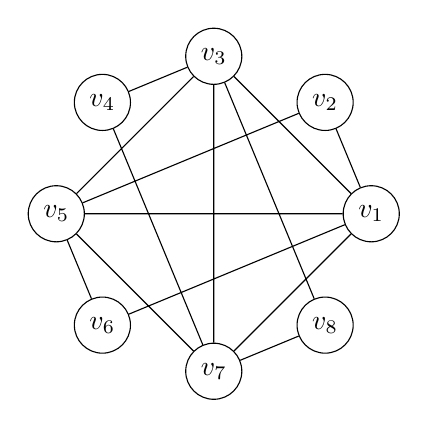
\begin{tikzpicture}[scale=2, bend angle=22.5]
\tikzstyle{every node}=[draw,shape=circle];
\foreach \i in {1,...,8}
{
\path (45*\i-45:1cm) node (v\i) {$v_\i$};
}
\draw
(v1) -- (v2) (v3) -- (v4) (v5) -- (v6) (v7) -- (v8)
(v1) -- (v3) (v3) -- (v5) (v5) -- (v7) (v7) -- (v1)
(v2) -- (v5) (v4) -- (v7) (v6) -- (v1) (v8) -- (v3)
(v1) -- (v5) (v3) -- (v7);
\end{tikzpicture}
\end{frame}

\begin{frame}[fragile]
	\begin{multicols}{2}
\inputminted[xleftmargin=1.5em]{latex}{tikz/binary_tree.tex}
	\end{multicols}
\end{frame}

\begin{frame}
	\centering
	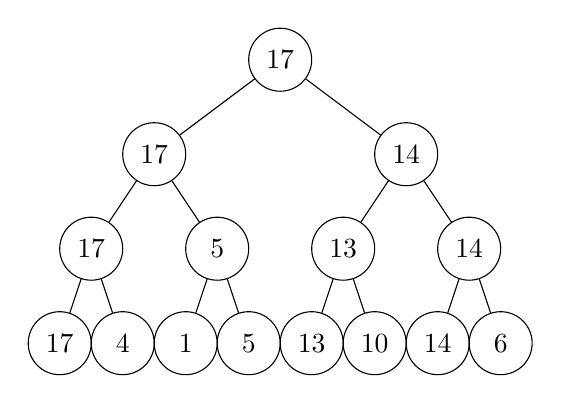
\begin{tikzpicture}[scale=0.8]
\tikzstyle{every node}=[draw,shape=circle,minimum size=0.8cm];
\node {17}[sibling distance=4cm]
child { node {17}[sibling distance=2cm]
	child {
		node {17}[sibling distance=1cm]
		child { node {17} }
		child { node {4} }
	}
	child {
		node {5}[sibling distance=1cm]
		child { node {1} }
		child { node {5} }
	}
}
child { node {14}[sibling distance=2cm]
	child {
		node {13}[sibling distance=1cm]
		child { node {13} }
		child { node {10} }
	}
	child {
		node {14}[sibling distance=1cm]
		child { node {14} }
		child { node {6} }
	}
};
\end{tikzpicture}
\end{frame}

\begin{frame}
The process of memorizing the code in TikZ is quite hard, so while you need to plot some graph with TikZ, it is highly recommended that you refer to the \myhref{http://www.texample.net/tikz/} for the codes of examples shown in it.
\end{frame}